\documentclass[letterpaper,11pt]{article}
\usepackage{graphicx}
\usepackage{latexsym}
\usepackage[empty]{fullpage}
\usepackage{titlesec}
\usepackage{marvosym}
\usepackage[usenames,dvipsnames]{color}
\usepackage{verbatim}
\usepackage{enumitem}
\usepackage[hidelinks]{hyperref}
\usepackage{fancyhdr}
\usepackage[english]{babel}
\usepackage{tabularx}
\usepackage{fontawesome5}
\usepackage{smartdiagram}
\usepackage{multicol}

\setlength{\multicolsep}{-3.0pt}
\setlength{\columnsep}{-1pt}
\input{glyphtounicode}
\pagestyle{fancy}
\fancyhf{} % clear all header and footer fields
\fancyfoot{}
\renewcommand{\headrulewidth}{0pt}
\renewcommand{\footrulewidth}{0pt}

% Adjust margins
\addtolength{\oddsidemargin}{-0.6in}
\addtolength{\evensidemargin}{-0.5in}
\addtolength{\textwidth}{1.19in}
\addtolength{\topmargin}{-.7in}
\addtolength{\textheight}{1.4in}
\urlstyle{same}
\raggedbottom
\raggedright
\setlength{\tabcolsep}{0in}

% Sections formatting
\titleformat{\section}{
  \vspace{-7pt}\scshape\raggedright\large\bfseries
}{}{0em}{}[\color{black}\titlerule \vspace{0pt}]

% Ensure that generate pdf is machine readable/ATS parsable
\pdfgentounicode=1

%%%%%%%%%%%%%%%%%%%%%%%%%%%%  Commands  %%%%%%%%%%%%%%%%%%%%%%%%%%%%
\newcommand{\resumeItem}[1]{
  \item\small{
    {#1 \vspace{-3pt}}
  }
}
\newcommand{\resumeSubheading}[4]{
  \vspace{-3pt}\item
    \begin{tabular*}{1.0\textwidth}[t]{l@{\extracolsep{\fill}}r}
      \textbf{#1} & \textbf{\small #2} \\
      \textit{\small#3} & \textit{\small #4} \\
    \end{tabular*}\vspace{-7pt}
}
\newcommand{\resumeSubheadingContinue}[2]{
  \vspace{-3pt}
    \begin{tabular*}{1.0\textwidth}[t]{l@{\extracolsep{\fill}}r}
      \textit{\small#1} & \textit{\small #2} \\
    \end{tabular*}\vspace{-7pt}
}
\newcommand{\resumeProjectHeading}[2]{
  \vspace{-3pt}\item
    \begin{tabular*}{1.0\textwidth}[t]{l@{\extracolsep{\fill}}r}
      \textbf{#1} & \textbf{\small #2} \\
    \end{tabular*}\vspace{-7pt}
}
\newcommand{\resumeSubItem}[1]{\resumeItem{#1}\vspace{0pt}}
\renewcommand\labelitemi{$\vcenter{\hbox{\tiny$\bullet$}}$}
\renewcommand\labelitemii{$\vcenter{\hbox{\tiny$\bullet$}}$}
\newcommand{\resumeSubHeadingListStart}{\begin{itemize}[leftmargin=0.0in, label={}]}
\newcommand{\resumeSubHeadingListEnd}{\end{itemize}}
\newcommand{\resumeItemListStart}{\begin{itemize}}
\newcommand{\resumeItemListEnd}{\end{itemize}\vspace{0pt}}

%%%%%%%%%%%%%%%%%%%%%%%%%%%%  Heading  %%%%%%%%%%%%%%%%%%%%%%%%%%%%
\begin{document}
    \begin{center}
        % NAME
        {\Huge\scshape Jason J. Evans} 
        % SUBHEADING
        \\Bioinformatics Engineer and Data Scientist\\
        \small
        % EMAIL
        \href{mailto:jason.j.evans@gmail.com}{\raisebox{-0.2\height}\faEnvelope\  \underline{jason.j.evans@gmail.com}} ~ 
        % LINKEDIN
        \href{https://www.linkedin.com/in/jasonjevans/}{\raisebox{-0.2\height}\faLinkedin\ \underline{linkedin.com/in/jasonjevans}}  ~
        % GITHUB
        \href{https://github.com/jjevans}{\raisebox{-0.2\height}\faGithub\ \underline{github.com/jjevans}} ~
		%phone
		\href{tel:12624420503}{\raisebox{-0.2\height}\faPhone\ \underline{262-442-0503}}
    \end{center}

%%%%%%%%%%%%%%%%%%%%%%%%%%%%  Education  %%%%%%%%%%%%%%%%%%%%%%%%%%%%


\section{\Large{Highlights}}
    \vspace{-7pt}
%thin outline box
	\fbox{\parbox{\linewidth}{

\begin{minipage}{-0.0\linewidth}
%image to left side of highlights
        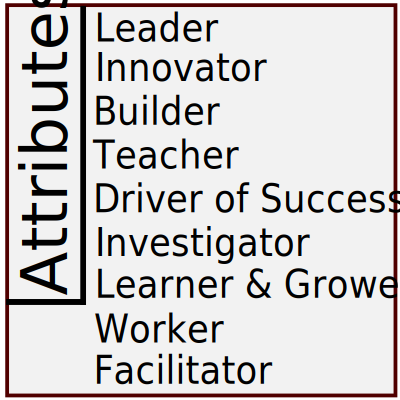
\includegraphics[scale=0.45]{resume_attributes.png}
\end{minipage}
\hfill
\begin{minipage}[c]{0.75\linewidth}
%bullet points of key info to right of image
	\begin{itemize}
	\small
	\item[$\bullet$] \textbf{15+ years work experience applying bioinformatics in biotechnology, academic, clinical settings}
	%\item[$\bullet$] \textbf{Significant experience handling and processing next-generation sequence in scalable big-data environments}
	\item[$\bullet$] \textbf{10+ years experience support and development in a CAP/CLIA genetic testing laboratory setting}
	\item[$\bullet$] \textbf{Designed and implemented variant calling and annotation pipelines for integration of exome and genome sequencing into clinical lab workflows}
	\item[$\bullet$] \textbf{Skilled on a Linux command-line for transform, merge, and extraction of complex data to reduce key information that is digestable to lab scientists and geneticists alike}

       \end{itemize}
\end{minipage}
	\vspace*{0mm}
}}
    \vspace{-0pt}
\section{\Large{Education}}
  \resumeSubHeadingListStart
  
    % MAIN INFORMATION
    \resumeSubheading
    {University of Wisconsin-Madison}{Madison, WI}
    {Bachelors of Science, Botany}{1999}
        % BULLET POINTS
%        \resumeItemListStart
%            \resumeItem{\textbf{Selected Coursework:} COURSES}
%            \resumeItem{\textbf{Awards:} AWARDS}
%        \resumeItemListEnd
  \resumeSubHeadingListEnd
 \resumeSubHeadingListStart
         \resumeSubheading
    {Medical College of Wisconsin and Marquette University}{Milwaukee, WI}
    {Masters of Science, Joint Program in Bioinformatics}{2009}    
  \resumeSubHeadingListEnd


%%%%%%%%%%%%%%%%%%%%%%%%%%%%  Experience  %%%%%%%%%%%%%%%%%%%%%%%%%%%%
    \vspace{-0pt}
\section{\Large{Experience}}

    \resumeSubHeadingListStart
    
        % COMPANY 1
        \resumeSubheading
        {Quest Diagnostics}{Marlborough, MA}
            % POSITION 1
            {\textbf{Sr. Manager, Bioinformatics, Clinical Operations}}{12/2021-Current}
            \resumeItemListStart
                \resumeItem{Established a dedicated Clinical Operations group in support of Clinical Geneticists, Variant Scientists and Lab Operations within a CAP/CLIA regulatory setting}
                \resumeItem{Led development for cloud-based systems and the tools to register and find data, track provenance, and ease troubleshooting of cloud pipelines and supporting systems}
                \resumeItem{Drove extensible implementation of Python libraries to standardize logging, tracking, and connection between LIMS, cloud-based systems and interpretation and reporting databases}
                \resumeItem{Consolidated and simplified support of all of our systems used in our production clinical setting}
            \resumeItemListEnd

            % POSITION 2
            \resumeSubheadingContinue
            {\textbf{Sr. Staff Scientist, Bioinformatics, Research \& Development}}{7/2019-12/2021}
            \resumeItemListStart
                \resumeItem{Built first-in-kind long-read sequencing assay for quantification of tandem repeats for Ataxia diagnostic}
                \resumeItem{Built high-throughput whole exome pipeline for large scale consumer-based assay processing 100,000 samples per year}
            \resumeItemListEnd
            
            % POSITION 3
            \resumeSubheadingContinue
            {\textbf{Sr. Scientist, Bioinformatics, Research \& Development}}{1/2018-7/2019}
            \resumeItemListStart
                \resumeItem{Established the systems needed to scale from small targeted panel assays to assays using a Whole Exome Sequencing backbone for diagnostic use}
                \resumeItem{Produced Whole Exome Sequencing Copy Number Variant caller using a coverage-based approach}
            \resumeItemListEnd
  

        % COMPANY 2
        \resumeSubheading
        {Courtagen Life Sciences}{Woburn, MA}
            % POSITION 1
            {\textbf{Bioinformatics Scientist, Annotation \& Interpretation}}{11/2015-7/2017}
            \resumeItemListStart
                \resumeItem{Support and implementation of interpretation and reporting web application providing feature improvements and bug fixes in a CAP/CLIA genetic testing environment}
                \resumeItem{Built web interface and backend to identify and queue variant confirmations using Sanger sequencing}
            \resumeItemListEnd
            

        % COMPANY 3
        \resumeSubheading
        {Laboratory of Molecular Medicine/Partners Personalized Medicine}{Cambridge, MA}
            % POSITION 1
            {\textbf{Bioinformatician}}{9/2012-11/2015}
            \resumeItemListStart
                \resumeItem{Produced end-to-end pipeline for distributed computation and variant calling for Whole Genome Sequencing in a CAP/CLIA genetic testing laboratory setting}
                \resumeItem{Implemented software to interface variant databases, variant annotation, and interpretation interfaces into a single, simple set of tools and resources}
            \resumeItemListEnd

    \resumeSubHeadingListEnd

%page end
\clearpage

%start new page
    \begin{center}
        % NAME
        {\Huge\scshape Jason J. Evans} 
        % SUBHEADING
        \\Bioinformatics Engineer and Data Scientist\\
        \small
        % EMAIL
        \href{mailto:jason.j.evans@gmail.com}{\raisebox{-0.2\height}\faEnvelope\  \underline{jason.j.evans@gmail.com}} ~ 
        % LINKEDIN
        \href{https://www.linkedin.com/in/jasonjevans/}{\raisebox{-0.2\height}\faLinkedin\ \underline{linkedin.com/in/jasonjevans}}  ~
        % GITHUB
        \href{https://github.com/jjevans}{\raisebox{-0.2\height}\faGithub\ \underline{github.com/jjevans}} ~
		%phone
		\href{tel:12624420503}{\raisebox{-0.2\height}\faPhone\ \underline{262-442-0503}}
    \end{center}
\section{\Large{Experience (con'd)}}
    \resumeSubHeadingListStart
    
        % COMPANY 4
        \resumeSubheading
        {Harvard School of Public Health, Bioinformatics Core}{Boston, MA}
            % POSITION 1
            {\textbf{Bioinformatician}}{7/2011-8/2012}
            \resumeItemListStart
                \resumeItem{Provided bioinformatics analyses and reports in support of contracting labs throughout HSPS}
                \resumeItem{Extensive contribution of tools and workflows towards the HSPS fork of the Galaxy Project}
            \resumeItemListEnd

        % COMPANY 4
        \resumeSubheading
        {Marquette University, School of Biology}{Milwaukee, WI}
            % POSITION 1
            {\textbf{Research Associate, Molecular Biology}}{5/2007-1/2008}
            \resumeItemListStart
                \resumeItem{Built molecular biology constructs for RNA Interference in \textit{Chlamydomonas}}
            \resumeItemListEnd


%%%%%%%%%%%%%%%%%%%%%%%%%%%%  PROJECTS  %%%%%%%%%%%%%%%%%%%%%%%%%%%%
%\section{Personal Projects} 
%    \resumeSubHeadingListStart

        % Project 1
%        \resumeProjectHeading
%        {PROJECT NAME -\href{LINK}{\raisebox{-0.2\height}\ \underline{LINK}}}
%        % Date
 %       {DATE}
 %       \resumeItemListStart
%            \resumeItem{WHAT YOU DID}
%        \resumeItemListEnd
    
%        % Project 2
%        \resumeProjectHeading
%        {PROJECT NAME -\href{LINK}{\raisebox{-0.2\height}\ \underline{LINK}}}
%       % Date
%        {DATE}
%        \resumeItemListStart
%            \resumeItem{WHAT YOU DID}
%        \resumeItemListEnd
        
%    \resumeSubHeadingListEnd


        % COMPANY 5
        \resumeSubheading
        {Applied Biosystems}{Foster City, CA}
            % POSITION 1
            {\textbf{Bioinformatics Scientist}}{5/2001-5/2005}
            \resumeItemListStart
                \resumeItem{Built the computational analysis and system to run it in support of SNPlex custom oligo array}
                \resumeItem{Assisted in development of the first ABI 7900 high-throughput qPCR platform.  Provided continued improvements in basecalling for the ABI 3700 sequencing instrument}
				\resumeItem{Leveraged the Celera human genome draft to identify putative drug targets in collaboration with contracted pharmaceutical companies}
            \resumeItemListEnd   
            
        % COMPANY 6
        \resumeSubheading
        {Celera Genomics}{Foster City, CA}
            % POSITION 1
            {\textbf{Scientist}}{5/2000-5/2001}
            \resumeItemListStart
                \resumeItem{Wet lab identification of full-length cDNA clones targeting putative drug targets}
                \resumeItem{cDNA library archival in a high-throughput cloning laboratory focused on isolating drug targets identified by draft genome}
            \resumeItemListEnd   
    \resumeSubHeadingListEnd

%%%%%%%%%%%%%%%%%%%%%%%%%%%%  Publications  %%%%%%%%%%%%%%%%%%%%%%%%%%%%
\section{\Large{Publications}}
	\begin{itemize}[leftmargin=0.15in, label={}]
		\small{\item{Tsai, E.A.; Shakbatyan, R.; Evans, J.; Rossetti, P.; Graham, C.; Sharma, H.; Lin, C.-F.; Lebo, M.S. \textbf{Bioinformatics Workflow for Clinical Whole Genome Sequencing at Partners HealthCare Personalized Medicine}. J. Pers. Med. 2016, 6, 12.}}
	\end{itemize}


%outline box
%\vspace*{4mm}

\section{\Large{Skills}}
%\fbox{\parbox{\linewidth}{
%\vspace*{1mm}
\begin{minipage}{0.43\linewidth}
\fbox{\parbox{\linewidth}{
%\vspace*{1mm}
\begin{flushleft}\Large{\textbf{Leadership Style}}\end{flushleft}
\vspace*{-1mm}
\smartdiagramset{description title width=2.5cm, description title text width=2.5cm,}
\smartdiagram[descriptive diagram]{
{\small{Example},Lead by showing the way we do business},
{\small{Conversation}, Lead in question and answer by working in a team dynamic},
{\small{Coaching}, Nurture and teaching leads to creative solutions},
{\small{Transformation}, Inspire through understanding our future},
}}}
\end{minipage}
\hfill
\begin{minipage}[c]{0.55\linewidth}
%    \vspace{-7pt}
\fbox{\parbox{\linewidth}{ 
\begin{flushleft}\Large{\textbf{Technical}}\end{flushleft}
   \begin{itemize}
    [leftmargin=0.15in, label={}]\small{\item{
        % LANGUAGES
        \textbf{Languages}{: STUFF} \\
        % TOOLS
        \textbf{Developer Tools}{: STUFF} \\
        % TECHNOLOGIES
        \textbf{Technologies/Frameworks}{: STUFF} \\}}
    \end{itemize}
}}
	\vspace*{0mm}
\end{minipage}
%box around skills
%}}
\end{document}
